% Title: gl2ps_renderer figure
% Creator: GL2PS 1.4.2, (C) 1999-2020 C. Geuzaine
% For: Octave
% CreationDate: Tue Oct 26 12:45:11 2021
\setlength{\unitlength}{1pt}
\begin{picture}(0,0)
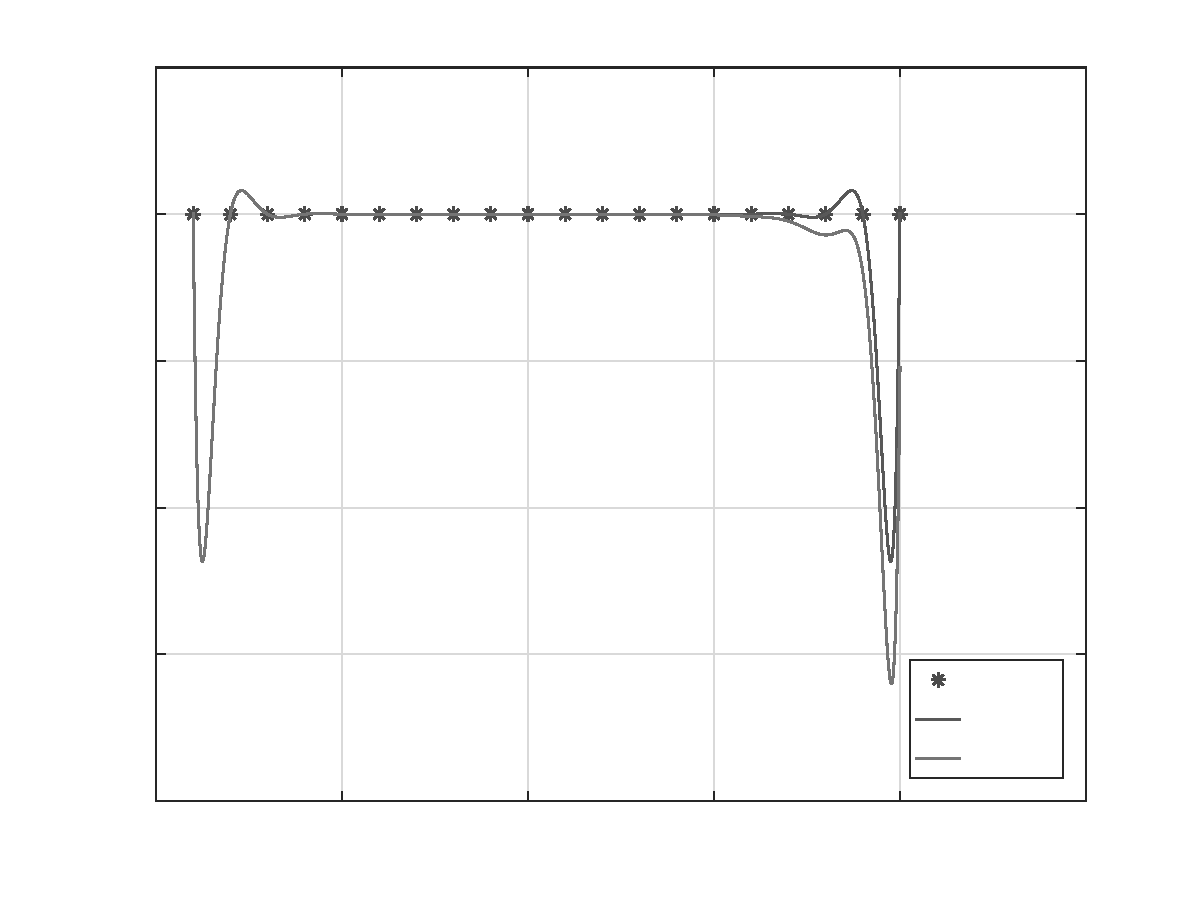
\includegraphics[scale=1]{figures/chap08/OUT/WilkinsonPlotGray-inc}
\end{picture}%
\begin{picture}(576,432)(0,0)
\fontsize{10}{0}\selectfont\put(74.8799,40.0181){\makebox(0,0)[t]{\textcolor[rgb]{0.15,0.15,0.15}{{0}}}}
\fontsize{10}{0}\selectfont\put(164.16,40.0181){\makebox(0,0)[t]{\textcolor[rgb]{0.15,0.15,0.15}{{5}}}}
\fontsize{10}{0}\selectfont\put(253.44,40.0181){\makebox(0,0)[t]{\textcolor[rgb]{0.15,0.15,0.15}{{10}}}}
\fontsize{10}{0}\selectfont\put(342.72,40.0181){\makebox(0,0)[t]{\textcolor[rgb]{0.15,0.15,0.15}{{15}}}}
\fontsize{10}{0}\selectfont\put(432,40.0181){\makebox(0,0)[t]{\textcolor[rgb]{0.15,0.15,0.15}{{20}}}}
\fontsize{10}{0}\selectfont\put(521.28,40.0181){\makebox(0,0)[t]{\textcolor[rgb]{0.15,0.15,0.15}{{25}}}}
\fontsize{10}{0}\selectfont\put(69.8755,47.52){\makebox(0,0)[r]{\textcolor[rgb]{0.15,0.15,0.15}{{-2e+16}}}}
\fontsize{10}{0}\selectfont\put(69.8755,117.936){\makebox(0,0)[r]{\textcolor[rgb]{0.15,0.15,0.15}{{-1.5e+16}}}}
\fontsize{10}{0}\selectfont\put(69.8755,188.352){\makebox(0,0)[r]{\textcolor[rgb]{0.15,0.15,0.15}{{-1e+16}}}}
\fontsize{10}{0}\selectfont\put(69.8755,258.768){\makebox(0,0)[r]{\textcolor[rgb]{0.15,0.15,0.15}{{-5e+15}}}}
\fontsize{10}{0}\selectfont\put(69.8755,329.184){\makebox(0,0)[r]{\textcolor[rgb]{0.15,0.15,0.15}{{0}}}}
\fontsize{10}{0}\selectfont\put(69.8755,399.6){\makebox(0,0)[r]{\textcolor[rgb]{0.15,0.15,0.15}{{5e+15}}}}
\fontsize{11}{0}\selectfont\put(298.08,27.0181){\makebox(0,0)[t]{\textcolor[rgb]{0.15,0.15,0.15}{{$t$}}}}
\fontsize{11}{0}\selectfont\put(23.8755,223.56){\rotatebox{90}{\makebox(0,0)[b]{\textcolor[rgb]{0.15,0.15,0.15}{{$p(t)$}}}}}
\fontsize{11}{0}\selectfont\put(298.08,409.6){\makebox(0,0)[b]{\textcolor[rgb]{0,0,0}{{The Wilkinson polynomial and its perturbation}}}}
\fontsize{9}{0}\selectfont\put(463.907,105.637){\makebox(0,0)[l]{\textcolor[rgb]{0,0,0}{{roots}}}}
\fontsize{9}{0}\selectfont\put(463.907,86.7788){\makebox(0,0)[l]{\textcolor[rgb]{0,0,0}{{$p_W$}}}}
\fontsize{9}{0}\selectfont\put(463.907,67.9214){\makebox(0,0)[l]{\textcolor[rgb]{0,0,0}{{$\tilde{p}_W$}}}}
\end{picture}
